\documentclass[11pt]{article}
\usepackage{graphicx}

\begin{document}
	\begin{center}
		\begin{Large}
			Assignment No 4
		\end{Large}
	\end{center}•
	Aim: Generating intermediate Code for assignment statement using LEX and YACC.\\
	
	\noindent
	Objective:
	\begin{enumerate}
		\item To understand fourth phase of compiler: Intermediate code generation.
		\item To learn and use compiler writing tools.
		\item To learn how to write three address code for given assignment statement.
	\end{enumerate}•
	
	\noindent
	Software Requirement:
	\begin{enumerate}
		\item Linux Operating System
		\item Lex compiler
		\item Yacc compiler
	\end{enumerate}•
	
	\noindent
	Mathematical Model:\\
	Consider a set S consisting of all the elements related to a program.The mathematical model is given as below,\\
	S={s,e,X,Y,Fme,DD,NDD,Mem shared}\\ Where, s = Initial State \\e = End State\\
	X	= Input data.Here it is assignment statement.\\
	Y	= Output.Here output is intermediate code for assignment statement.\\
	Fme = Algorithm/Function used in program.for eg.{addquad(),display()}\\
	DD = Deterministic Data\\
	NDD = Non deterministic Data\\
	
	
	\begin{center}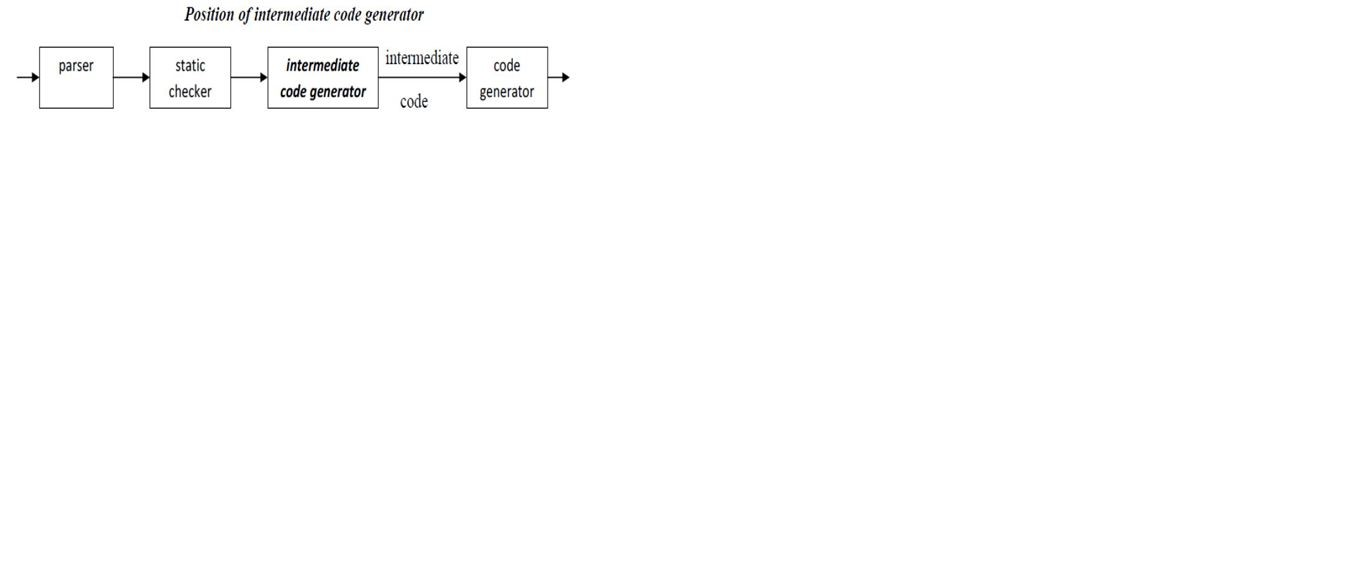
\includegraphics{temp.png}
	\end{center}•
	
	
	\noindent
	THEORY :\\
	Introduction:\\
	In the analysis-synthesis model of a compiler, the front end analyzes a source program and creates an intermediate representation, from which the back end generates target code. Ideally, details of the source language are confined to the front end, and details of the target machine to the back end. The front end translates a source program into an intermediate representation from which the back end generates target code.With a suitably defined intermediate representation, a compiler for language i and machine j can then be built by combining the front end for language i with the back end for machine j. This approach to creating suite of compilers can save a considerable amount of effort: m x n compilers can be built by writing just m front ends and n back ends.\\
	
	\noindent
	Benefits of using a machine-independent intermediate form are:\\
	\begin{enumerate}
		\item Retargeting is facilitated. That is, a compiler for a different machinecan be created by attaching a back end for the new machine to an existing front end.
		\item A machine-independent code optimizer can be applied to the intermediate representation.
	\end{enumerate}•
	
	\noindent
	Intermediate Languages:\\
	Three ways of intermediate language representation:\\
	\begin{enumerate}
		\item Syntax Tree:\\
		A syntax tree depicts the natural hierarchical structure of a source program. A dag (Directed Acyclic Graph) gives the same information but in a more compact way because common subexpressions.\\
		\begin{center}
			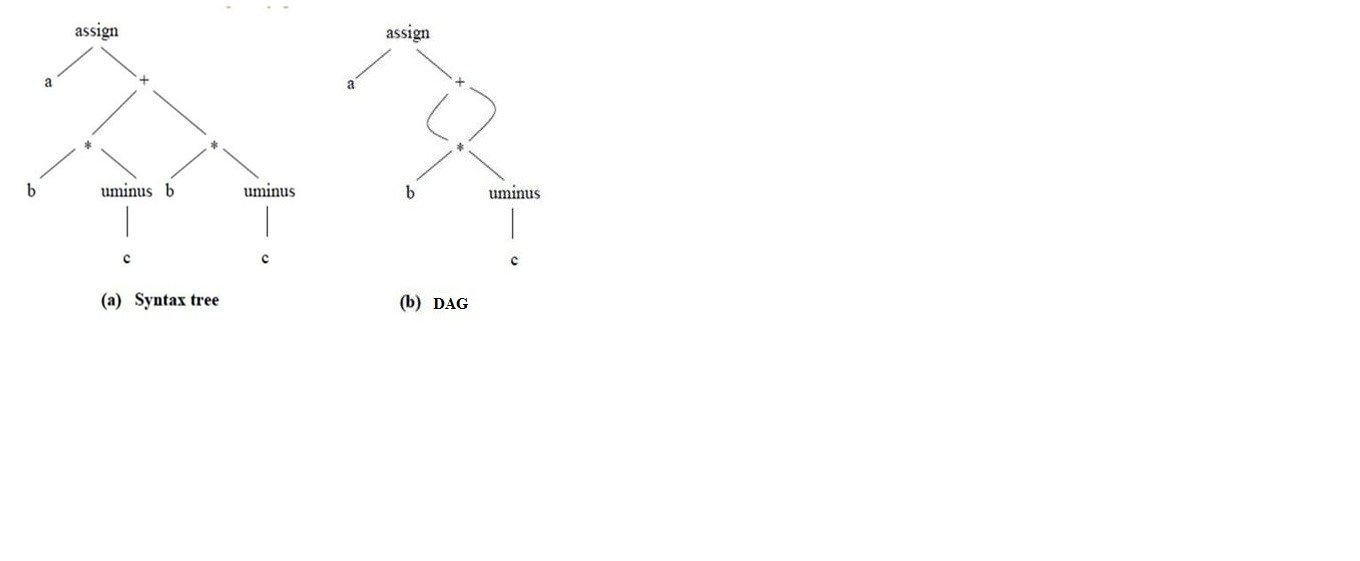
\includegraphics{syntax.png}
		\end{center}•
		
		\item Postfix notation\\
		Postfix notation is a linearized representation of a syntax tree; it is a list of the nodes of the tree in which a node appears immediately after its children. The postfix notation for the syntax tree given above
		is, a b c uminus * b c uminus $* +$ assign
		
		\item Three Address Code\\
		Three-address code is a sequence of statements of the general form,\\
		$$x: = y op z$$
		where x, y and z are names, constants, or compiler-generated temporaries; op stands for any operator, such as a fixed- or floating-point arithmetic operator, or a logical operator on Boolean valued data. Thus a source language expression like x+ y*z might be translated into a sequence,\\
		
		$$t1 : = y * z$$ 
		$$t2 : = x + t1 $$
		where t1 and t2 are compiler-generated temporary names. The reason for the term three-address code is that each statement usually contains three addresses, two for the operands and one for the result.\\
	\end{enumerate}•
	
	\noindent
	Types of Three-Address Statements :\\
	\begin{enumerate}
		\item Assignment Statements: X:$=$ Y op Z
		\item Unary Assignment Statements: X:$=$ op Z
		\item Copy Statements: X:$=$ Y
		\item Unconditional Jump: goto L,with L a label of a statement.
		\item Conditional Juml: if X relop Y goto L
		\item Procedure Call: param x, and call p,n for caling a procedure,p,with nparameters.return Y is the returned value of the procedure:\\
		param x1 param x2\\
		$...$\\
		param xn\\
		call p,n\\
		\item Indexed Assignments: X:=Y[i] or x[i]:=Y
		\item Pointer Assignments: X:=\&Y,X:$=*$Y,or *X:$=$Y;where \&Y stands for the address of Y, and *Y the value of Y.
		
	\end{enumerate}•
	
	\noindent
	Translation scheme for Assignment Statement :\\
	Consider the following grammar for assignment statement.\\
	S $-> $id=E\\
	E $->$ E1 + E2\\
	E $->$ E1 * E2\\
	E $->$ -E1\\
	E $->$ (E1)\\
	E $->$ id\\
	
	\noindent
	Advantages of three-address code :\\
	\begin{enumerate}
		\item The unraveling of complicated arithmetic expressions and of nestedflow-of-control statements makes three-address code desirable for target code generation and optimization.
		\item The use of names for the intermediate values computed by a programallows three address code to be easily rearranged unlike postfix notation.
	\end{enumerate}•
	
	\noindent
	Command\\ :
	\$ lex $<$program name$>$.l\\
	\$ yacc -d $<$program name$>$.y\\
	\$ gcc lex.yy.c y.tab.c -ll -ly\\
	\$ ./a.out$<$input.txt\\
	
	\noindent
	CONCLUSION :\\
	Thus, we have implemented LEX and YACC program to generate an intermediate code for assignment statement.\\
	
	\begin{center}
		\begin{tabular}{|c|c|c|c|c|}
			•$Roll$ $No$ & $Name$ $of$ $Student$ & $Date$ $of$ $performance$ & $Date$ $of$ $Checking$ & $Signature$ $of$ $Staff$ \\ \hline
			$BECOC357$ & Sunny Shah& 01 / 09 / 2017& 20 / 09 / 2017 & \\ \hline
		\end{tabular}•
	\end{center}•
	\newpage
	\section{PLAGARISM REPORT :}
	\begin{figure}[h!]
		\centering
		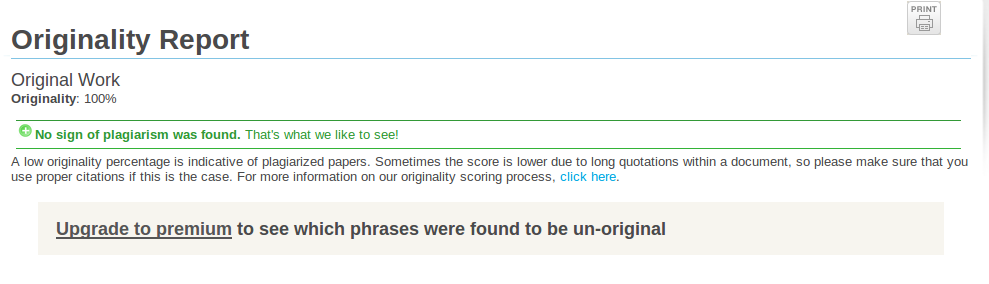
\includegraphics[height=5in,width=6in]{plagiarism4.png}
		\caption{Plagarism Checker www.smallseotools.com/plagarism-checker}
	\end{figure}
	\newpage
\end{document}
